\documentclass{IEEEjmw}

\usepackage[colorlinks,urlcolor=blue,linkcolor=blue,citecolor=blue]{hyperref}

\usepackage{color,array}

\usepackage{graphicx}
\usepackage{siunitx}

\usepackage{hyperref}
\hypersetup{
	colorlinks=true,
	linkcolor=blue,
	filecolor=magenta,      
	urlcolor=cyan,
	pdfpagemode=FullScreen,
}

%\jvol{00}
%\jnum{XX}
%\paper{1234567}
%\pubyear{2020}
%\receiveddate{September XX, 2020}
%\accepteddate{October XX, 2020}
%\publisheddate{November~XX, 2020}
%\currentdate{November~XX, 2020}
%\doiinfo{JMW.2020.Doi Number}

\newtheorem{theorem}{Theorem}
\newtheorem{lemma}{Lemma}
\setcounter{page}{1}
%% \setcounter{secnumdepth}{0}

%% Python listing def

\usepackage{listings}

\definecolor{codegreen}{rgb}{0,0.6,0}
\definecolor{codegray}{rgb}{0.5,0.5,0.5}
\definecolor{codepurple}{rgb}{0.58,0,0.82}
\definecolor{backcolour}{rgb}{0.95,0.95,0.92}

\lstdefinestyle{mystyle}{
	backgroundcolor=\color{backcolour},  
	commentstyle=\color{codegreen},
	keywordstyle=\color{magenta},
	numberstyle=\tiny\color{codegray},
	stringstyle=\color{codepurple},
	basicstyle=\footnotesize,
	breakatwhitespace=false,        
	breaklines=true,                
	captionpos=b,                   
	keepspaces=true,                
	numbers=left,                   
	numbersep=5pt,                 
	showspaces=false,               
	showstringspaces=false,
	showtabs=false,                 
	tabsize=2
}

\lstset{style=mystyle}


\begin{document}

%\sptitle{Article Category}

\title{scikit-rf - An Open Source Python Package for Microwave Network Creation, Analysis and Calibration} 

%\editor{The associate editor coordinating the review of this manuscript and approving it for publication\break was F. A. Author.}

\author{A. Arsenovic\affilmark{1}}
\affil{810 Labs LLC} 
\corresp{CORRESPONDING AUTHOR: A. Arsenovic (e-mail: \href{mailto:alex@810lab.com}{alex@810lab.com}).}

% After Alex, should we  proceed by GitHub contributor ranking or by alphabetical order ?
%
% GitHub list of contributors
% https://github.com/scikit-rf/scikit-rf/graphs/contributors

\author{J. Hillairet\affilmark{2}}
\affil{CEA, IRFM, F-13108 St-Paul-Lez-Durance, France} 

\author{J. Anderson\affilmark{3}}
\affil{Purdue University, West Lafayette, Indiana, USA}

\author{H. Forsten\affilmark{4}}
\affil{TBD} 

\author{Michael Eller\affilmark{5}}
\affil{University of Virginia, Virginia, USA}

\author{Noah Sauber\affilmark{5}}
\affil{University of Virginia, Virginia, USA}

\author{Robert Weikle\affilmark{6}}
\affil{TBD}

%%%%% Please add your name and affiliation here



%\authornote{This work was supported by ...}

\markboth{PREPARATION OF PAPERS FOR IEEE JOURNAL OF MICROWAVES}{A. ARSENOVIC {\itshape ET AL}}

\begin{abstract}
Measurements at microwave frequencies can require a  significant  amount post-processing  and  analysis,  especially  in research  and  prototyping environments.  From  our  experience, none  of   the   existing   software   products  satisfy   the   needs   of these environments in which the abilities to understand, modify, and  extend  existing  functionality  are  vital.  In  an  attempt  to provide this  needed  functionality,  we  have  created  scikit-rf;  an open  source,  BSD-licensed  package  for  microwave  engineering implemented   in   the   Python  programming   language.   scikit-rf seeks  to  provide  a  modern,  object-oriented  library  for  network analysis  and  calibration  aimed  at  being  flexible  and scalable. In  this  paper,  we  introduce  the  motivation  behind  the  scikit-rf  project   and   demonstrate  its  current   abilities   with   some applications.
\end{abstract}

\begin{IEEEkeywords}

\end{IEEEkeywords}

\maketitle

\section{Context and Motivations}
With the rapid proliferation of telecommunication and radio-frequency (RF) applications, so too has demand grown for tools to design and characterize these devices. Scikit-rf is a Python package designed to make RF/Microwave engineering both robust and approachable. The package provides a modern, object-oriented library for RF network analysis, circuit building and calibration. Besides offering standard microwave network operations, such as reading/writing Touchstone files (\texttt{.sNp} files), connecting or de-embedding N-port networks, frequency/port slicing, concatenation or interpolations, it is also capable of advanced operations such as Vector Network Analyzer (VNA) calibrations, time-gating, interpolating between an individual set of networks, deriving network statistical properties and supports Virtual Instrument for direct communication to VNAs. The package also allows straightforward plotting of rectangular plots (dB, mag, phase, group delay, etc), Smith Charts or automated uncertainty bounds.
 
The project was created in 2009 and has been continually developed since. The package is distributed under the Berkeley Software Distribution (BSD) licence and is actively developed by more than 40 volunteers on GitHub. The project has users in several universities and research institutes around the world as well as corporate users from large companies including Keysight, Rohde \& Schwarz, National Instruments, Nvidia, and 3M. As of 2021, the package has been downloaded more than 220,000 times since its creation and has been used in over thirty publications.

As the package is developed in Python, it makes it naturally compatible with the rich set of modern scientific Python libraries. Results can be shared and directly reproduced by other researchers using tools such as Binder or Google Colab. Being a python library, it is also naturally compatible with the robust testing and code coverage frameworks developed for the language, with reproducible modelling approaches using online virtualization services. Being open-source, users of scikit-rf are able to see exactly what the source code is doing and, if a feature does not exist, are able to freely contribute it to extend the library for their work and for others. And of course, it is free.

\section{Basics Usage of scikit-rf}

Detailed installation instructions can be found in the scikit-rf documentation (\url{https://scikit-rf.readthedocs.io/en/latest/}). For those familiar with Python, it is no different from installing any other package, being available through both pip and conda. The following sections outline some of the fundamental features of scikit-rf, and include code snippets to provide a starting point for new users.

\subsection{Reading and Plotting Networks}


The central object in the scikit-rf package is a N-port microwave Network object. A Network can be created in various ways, for example by reading a Touchstone file named \texttt{measured\_data.s2p}:

\begin{lstlisting}[language=Python]
>>> import skrf as rf
>>> example_network = rf.Network('measured_data.s2p')
\end{lstlisting}

In order for the reader to reproduce the given examples, a test-case is provided in the package and can be imported via:

\begin{lstlisting}[language=Python]
>>> from skrf.data import ring_slot
>>> ring_slot
2-Port Network: 'ring slot',  75.0-110.0 GHz, 201 pts, z0=[50.+0.j 50.+0.j]
\end{lstlisting}


The basic attributes of a microwave Network are provided by the following properties:
\begin{itemize}
\item \texttt{s}: Scattering parameter matrix.
\item \texttt{z0}: Port impedance matrix.
\item \texttt{frequency}: Frequency Object.
\end{itemize}

S-parameters are represented by a ($n_{bf} \times N \times N$) NumPy (\url{https://numpy.org/}) array\cite{harris2020}, where $n_{bf}$ is the number of frequency points and $N$ is the number of ports of the network. For example, to inspect the 2-by-2 S-parameters for the first frequency element:

\begin{lstlisting}[language=Python]
>>> ring_slot.s[0]  # or ring_slot.s[0,:]
array([[-0.50372318+0.4578448j ,  0.6134571 +0.36678139j],
[ 0.6134571 +0.36678139j, -0.19958433+0.6483347j ]])
\end{lstlisting}

The Network object has numerous other properties and methods which can found in  \href{https://scikit-rf.readthedocs.io}{the documentation}. If you are using IPython\cite{perez2007}, the Jupyter Notebook\cite{granger2021} or any advanced Python editor, then these properties and methods can be ‘tabbed’ out on the command line.

\begin{lstlisting}[language=Python]
>>> ring_slot.s<TAB>
ring_slot.s ring_slot.s_arcl
ring_slot.s11 ring_slot.s_arcl_unwrap ...
\end{lstlisting}

Plotting the ring slot’s scattering parameters on the Smith chart can be done in one line (figure~\ref{fig:figure1}).

\begin{lstlisting}[language=Python]
>>> from matplotlib import pyplot as plt
>>> %matplotlib inline # used in jupyter notebook
>>> ring_slot.plot_s_smith(lw=2)
>>> plt.xlim(-1,2)
\end{lstlisting}

\begin{figure}
	\centering
	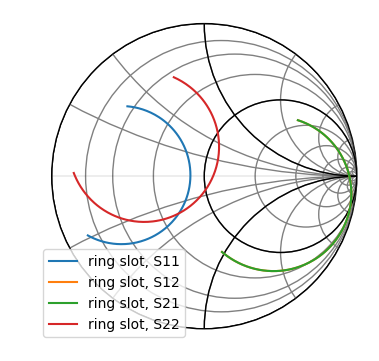
\includegraphics[width=0.95\linewidth]{figures/figure1}
	\caption{Scattering parameters of the \texttt{ring\_slot} Network plotted on a Smith chart}
	\label{fig:figure1}
\end{figure}

Frequency ranges of networks can also be selected by using human-readable strings, as you would array indices’. For instance, the following line will plot the log magnitude of $S_{11}$ for the frequency range of 80-90~GHz (figure~\ref{fig:figure2}), expressed in "natural" language:

\begin{lstlisting}[language=Python]
>>> ring_slot['80-90ghz'].plot_s_db(m=0, n=0)
\end{lstlisting}

\begin{figure}
	\centering
	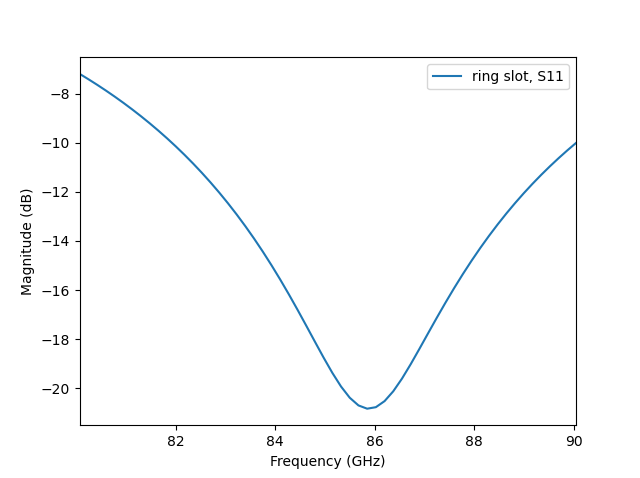
\includegraphics[width=0.95\linewidth]{figures/figure2}
	\caption{$S_{11}$ of \texttt{ring\_slot} Network plotted in log magnitude}
	\label{fig:figure2}
\end{figure}

Other parameters are accessible, such as impedance ($Z$), admittance ($Y$), transfer ($T$) or chain (ABCD) parameters using \texttt{ring\_slot.z}, \texttt{ring\_slot.y}, \texttt{ring\_slot.t} or \texttt{ring\_slot.a} respectively. Several other features related to network processing can be found in the scikit-rf documentation. The next sections illustrate a few of them. 

\subsection{Network Operations}
Element-wise mathematical operations on the scattering parameter matrices are accessible through overloaded operators. Hence, networks can be added, subtracted, multiplied along frequency and port axes. For example, to plot the complex difference between a \texttt{short} and a \texttt{delayshort}:

\begin{lstlisting}[language=Python]
>>> from skrf.data import wr2p2_short as short
>>> from skrf.data import wr2p2_delayshort as delayshort
>>> difference = (short - delayshort)
>>> difference.plot_s_mag(label='Mag of difference')
\end{lstlisting}

Another common application is calculating the phase difference between two networks using the division operator (\texttt{'/'}). 

\begin{lstlisting}[language=Python]
>>> (delayshort/short).plot_s_deg(label='Detrended Phase')
\end{lstlisting}

\subsection{Cascading and De-embedding}
scikit-rf supports the connection of arbitrary ports of N-port networks. Cascading and de-embedding 2-port networks with scikit-rf can also be done though the Python power operator (\texttt{'**'}). For example, to calculate a new 2-port network which is the cascaded connection of the two individual 2-port networks \texttt{line} and \texttt{short} (figure~\ref{fig:cascading}):

\begin{lstlisting}[language=Python]
>>> short = rf.data.wr2p2_short
>>> line = rf.data.wr2p2_line
>>> delayshort = line ** short
\end{lstlisting}

\begin{figure}
	\centering
	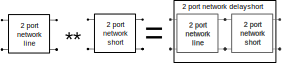
\includegraphics[width=0.95\linewidth]{figures/cascading}
	\caption{Cascading two 2-Port Networks in scikit-rf is easy with '**' operator in scikit-rf.}
	\label{fig:cascading}
\end{figure}

De-embedding can be accomplished by cascading the inverse of a network. The inverse of a network is accessed through the property \texttt{Network.inv} method. To de-embed the short from \texttt{delayshort}:

\begin{lstlisting}[language=Python]
>>> short_2 = line.inv ** delayshort
>>> short_2 == short
True
\end{lstlisting}

\begin{figure}
	\centering
	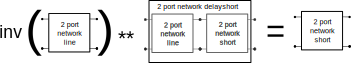
\includegraphics[width=0.95\linewidth]{figures/deembedding}
	\caption{Illustration of de-embedding using the inverse and cascade operators in scikit-rf.}
	\label{fig:deembedding}
\end{figure}

As seen in the previous example, Python comparison operators such as \texttt{'=='} also work with Networks. 

\subsection{Interpolation and concatenation}
A common need is to change the number of frequency points of a Network, for instance, to use the operators and cascading functions, the networks involved must have matching frequencies.

\begin{lstlisting}[language=Python]
>>> from skrf.data import wr2p2_line1 as line1
# next line fails due to the different network's frequencies
>>> line1 + line 
# next line is OK
>>> line.interpolate_from_f(line1.frequency) + line1  
\end{lstlisting}

A related application is the need to combine Networks which cover different frequency ranges. Two Networks can be concatenated (aka stitched) together using \texttt{stitch()}, which concatenates networks along their frequency axis. For example, to combine a WR-2.2 Network with a WR-1.5 Network:

\begin{lstlisting}[language=Python]
>>> from skrf.data import wr2p2_line, wr1p5_line
>>> big_line = rf.stitch(wr2p2_line, wr1p5_line)
>>> big_line
\end{lstlisting}

\subsection{Port Impedance renormalization}
S-parameters are defined for a given characteristic impedance $Z_0$. It can be necessary to renormalize S-parameters to a different $Z_0$ values. This example demonstrates how to use scikit-rf to renormalize a network's S-parameters to new port impedances. Although trivial, this example creates a matched load in \SI{50}{\ohm} and then re-normalizes to a \SI{25}{\ohm} environment, producing a reflection coefficient of 1/3. In case of complex characteristic impedances, scikit-rf supports both Power-Waves and Pseudo-Waves Scattering parameter definitions \cite{williams2013}.

\begin{lstlisting}[language=Python]
>>> match_at_50 = rf.wr10.match()
>>> match_at_50
1-Port Network: '',  75.0-110.0 GHz, 1001 pts, z0=[50.+0.j]
>>> match_at_50.s[0]  # S-parameter for the first frequency point
array([[0.+0.j]])
>>> match_at_50.renormalize(25)
>>> match_at_50
1-Port Network: '',  75.0-110.0 GHz, 1001 pts, z0=[25.+0.j]
>>> match_at_50.s[0]
array([[0.33333333+0.j]])
\end{lstlisting}

\section{Calibration}
It is possible with scikit-rf to calibrate a device under test (DUT), assuming that an acceptable set of standards have been preliminarily measured and have a corresponding set of ideal responses. This may be referred to as \textit{offline} calibration, because it is not occurring on-board the VNA itself. One benefit of this technique is that it provides maximum flexibility for non-conventional calibrations, and preserves all raw data. Self-calibration algorithms, such as Thru-Reflect-Line (TRL)\cite{engen1979}, do not require predefined ideal responses.

Several calibration routines are available in scikit-rf, for single port, two-ports or multi-ports Networks. Traditional 12 \cite{marks1997} or 16-terms \cite{silvonen1993} error models are available, but also 8-terms models \cite{speciale1977}, Short-Open-Load-Thru (SOLT) \cite{kruppa1971}, overdetermined one-port \cite{bauer1974}, Unknown-Thru \cite{ferrero1992}, Short-Delay-Delay-Load (SDDL) \cite{liu2006} or some special algorithms developed by our contributors. In some cases, it may be necessary or desirable to use a one-port network analyser to determine the full S-parameters of a two-port device. This technique is called one-port two-tier calibration \cite{ou2005} and is also implemented in scikit-rf. A complete list can be found on the scikit-rf website, and only a single one-port is given as an example in this section.

\subsection{One-Port Example}
A calibration in scikit-rf is generated using the \texttt{Calibration} object. In General, \texttt{Calibration} objects require two arguments: a list of measured Network’s and a list of ideal Network’s. The following example assumes that a set of measured and ideal networks are stored in separate directories named ideals and measured, for example a conventional short-open-load (SOL) calibration kit. These are used to create a One-Port \texttt{Calibration} and correct a measured DUT:

\begin{lstlisting}[language=Python]
import skrf as rf
from skrf.calibration import OnePort
# reads all Touchstone files located in the specified directory
my_ideals = rf.load_all_touchstones_in_dir('ideals/')
my_measured = rf.load_all_touchstones_in_dir('measured/')
# create a Calibration instance
cal = rf.OnePort(\
ideals = [my_ideals[k] for k in ['short','open','load']],
measured = [my_measured[k] for k in ['short','open','load']],
)
# run calibration algorithm
cal.run()
# apply it to a DUT
dut = rf.Network('my_dut.s1p')
dut_caled = cal.apply_cal(dut)
\end{lstlisting}

%\subsection{Two-Port Calibrations}
%Two-port calibrations are more involved than one-port. scikit-rf supports a few different two-port algorithms. The traditional SOLT algorithm uses the 12-term error model. This algorithm is straightforward, and similar to the \texttt{OnePort} example. The \texttt{EightTerm} calibration is based on the algorithm described in \cite{speciale1977}. It can be constructed from any number of standards, providing that some fundamental constraints are met. In short, you need three two-port standards; one must be transmissive, and one must provide a known impedance and be reflective. Note, that the word 8-term is used in the literature to describe a specific error model used by a variety of calibration algorithms, like TRL, LRM, etc. The \texttt{EightTerm} class, is an implementation of the algorithm cited above, which does not use any self-calibration.

\subsection{Multi-Line TRL Calibration}
scikit-rf can also be used for wideband Thru-Reflect-Line (TRL) calibration using multiple lines \cite{marks1991}. The necessary calibration standards in TRL calibration are at least two lines with different lengths and one or more reflective standards. Exact responses of the lines or reflects doesn’t need to be known because they are solved during the calibration. Ordinary SOLT or LRRM \cite{davidson1990} calibration usually moves the reference plane after the calibration to the SMA connector or probe tip used to contact the calibration standards. TRL calibration can be used to move the reference planes to the transmission lines on the substrate being measured if every measured standard includes a similar launch to the transmission lines. This makes TRL calibration very useful when accurate short, open, load and thru standards can’t be made, or when the measurement reference plane should be on the substrate being measured. 

\section{Time Domain and Gating}
Time-gating is a processing technique which is commonly used to pinpoint a response of interest in the presence of multiple reflections, eventually in order to isolate its effects \cite{cronson1973, bennett1978}. Commonly, this is done on-board a VNA. However, if instead the time-gating occurs offline on a computer, the user can keep the measurements separate from the processed results. This is important so that the processing algorithm can be altered in the future without re-taking data. 

In the following example, the time-gating functions of scikit-rf are used to filter out the effects of an undesired reflection. This can be done by using the method \texttt{Network.time\_gate}, and provide it an appropriate centre and span (in nanosecond). To see the effects of the gate, both the original and gated response are compared in the figure~\ref{fig:gated1}:

\begin{lstlisting}[language=Python]
>>> # probe_s11 and s11 data are available in the scikit-rf documentation
>>> probe_s11_gated = probe_s11.time_gate(center=0, span=.2)
>>> probe_s11_gated.name='gated probe'
>>> s11.plot_s_db_time()
>>> s11_gated.plot_s_db_time()
\end{lstlisting}

\begin{figure}
	\centering
	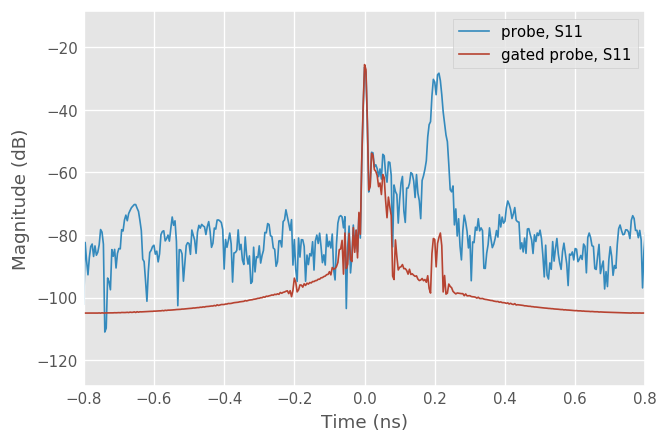
\includegraphics[width=0.95\linewidth]{figures/time_domain1}
	\caption{time-domain response of the original measurement and of the time-gated one.}
	\label{fig:gated1}
\end{figure}


The original $S_{11}$, blue curve in figure~\ref{fig:timedomain1}, shows an interference pattern due to this undesirable reflection at \SI{0.2}{\nano\second}. After gating, the probe response is cleaned and can be compared to the original one (red curve in figure~\ref{fig:timedomain1}):

\begin{lstlisting}[language=Python]
>>> s11.plot_s_db()
>>> s11_gated.plot_s_db()
\end{lstlisting}

\begin{figure}
	\centering
	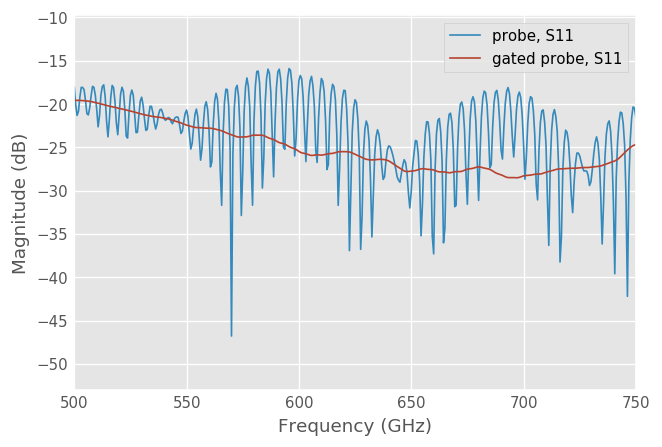
\includegraphics[width=0.95\linewidth]{figures/gated1}
	\caption{Comparison of the original $S_{11}$ response with the time-gated one.}
	\label{fig:timedomain1}
\end{figure}


\section{Circuit Building}
scikit-rf allows one to build a circuit of arbitrary topology, consisting of an arbitrary number of N-ports Networks connected together. Like in an electronic circuit simulator, the circuit must have one (or more) port(s) connected to the circuit. The \texttt{Circuit} object allows one retrieving the final $M$-ports Network (and thus its network parameters: $S$, $Z$, etc.), where $M$ is the number of ports defined. Moreover, the \texttt{Circuit} object also allows calculating the scattering matrix $S$ of the entire circuit, that is the "internal" scattering matrices for the various intersections in the circuit. The calculation algorithm is based on ref \cite{hallbjorner2003}.

The figure~\ref{fig:circuit} illustrates a network with 2 ports, Network elements $N_i$ and intersections. In order to define such circuit, one should define its connexion list, which describes how networks are interconnected to each other and to which ports, such as:
\begin{lstlisting}[language=Python]
connexions = [
[(network1, network1_port_nb), (network2, network2_port_nb), (network2, network2_port_nb), ...], 
...
]
\end{lstlisting}

For example, the connexion list to construct the circuit illustrated in figure~\ref{fig:circuit} could be:

\begin{lstlisting}[language=Python]
>>> connexions = [
[(port1, 0), (network1, 0), (network4, 0)],
[(network1, 1), (network2, 0), (network5, 0)],
[(network1, 2), (network3, 0)],
[(network2, 1), (network3, 1)],
[(network2, 2), (port2, 0)],
[(network5, 1), (ground1, 0)]
]
\end{lstlisting}

where we have assumed that \texttt{port1}, \texttt{port2}, \texttt{ground1} and all the \texttt{network1} to \texttt{network5} are scikit-rf Networks objects with same Frequency. Networks can have different (real) characteristic impedances: mismatch are taken into account. Note that the port 1 of the \texttt{network4} is left open, so is not described in the connexion list. Once the connexion list is defined, the \texttt{Circuit} is built with:

\begin{lstlisting}[language=Python]
resulting_circuit = rf.Circuit(connexions)
\end{lstlisting}

The resulting 2-ports Network is obtained with the \texttt{Circuit.network} parameter:
\begin{lstlisting}[language=Python]
resulting_network = resulting_circuit.network
\end{lstlisting}

Note that it is also possible to create manually a circuit of multiple Network objects using the connecting methods of scikit-rf. Although the \texttt{Circuit} approach to build a multiple Network may appear to be more verbose than the "classic" way for building a circuit, as the circuit complexity increases, in particular when components are connected in parallel, the \texttt{Circuit} approach is interesting as it increases the readability of the code. Moreover, a \texttt{Circuit}'s topology can be plotted using its \texttt{plot\_graph} method, which is useful to rapidly control if the circuit is built as expected.

\begin{figure}
	\centering
	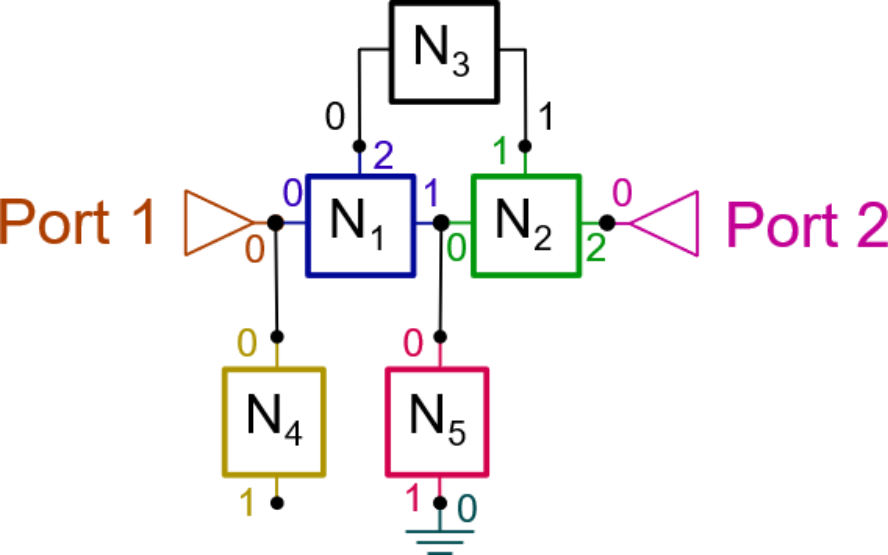
\includegraphics[width=0.95\linewidth]{figures/circuit}
	\caption{ Example of a Circuit made of various kinds of N-port Networks
		Summary}
	\label{fig:circuit}
\end{figure}

\section{Conclusion}
scikit-rf is an open-source Python package produced for RF/Microwave engineering. The package provides a modern, object-oriented library for RF network analysis, circuit building and calibration. Below is a current non-exhaustive feature list of scikit-rf (as of version 0.18).

\begin{itemize}
	\item	Microwave network operations
	\begin{itemize}
	\item	Read/Write touchstone (.sNp) files
	\item	S/Z/Y/ABCD/T - parameter conversions
	\item	Arithmetic operations on scattering parameters
	\item   Mixed mode and single ended port conversion
	\item	Cascade/De-embed Networks
	\item	Frequency and port slicing and concatenation.
	\item   Assembly of multiple-port networks
	\item    Vector fitting of equivalent circuit to S-parameters with SPICE netlist export
	\end{itemize}
\item	Sets of Networks:
	\begin{itemize}
		\item Statistical properties of a set of Network
		\item Interpolation between a set of Network (frequency or parametric)
		\item Methods to sort and visualize set behaviour
	\end{itemize}
\item	Plotting abilities:
	\begin{itemize}
		\item Rectangular plots (dB, mag, phase, group delay)
		\item Smith chart
		\item Automated uncertainty bounds
	\end{itemize}
\item	Calibration Routines:
	\begin{itemize}
		\item One-Port: SOL, Least Squares, SDDL
		\item Two-Port: TRL, Multiline TRL, SOLT, Unknown Thru, 8/16-Term
		\item Partial : Enhanced Response, One-Port Two-Path
	\end{itemize}
\item	Virtual Instruments (completeness varies by model)
	\begin{itemize}
		\item VNAs: PNA, PNAX, ZVA, HP8510, HP8720
		\item SA: HP8500
		\item Others: ESP300
	\end{itemize}
\item	Transmission Line Physics:
	\begin{itemize}
		\item Distributed Circuit, Coaxial/Coplanar/Rectangular/Circular Waveguides, Freespace, 
		\item Transmission line voltage, current, power and losses calculations
		\item Complex characteristic impedance support
	\end{itemize}

\end{itemize}

In addition to these rich features, there are also GUIs for time gating and sNp file viewing, with source code available at \url{https://github.com/scikit-rf/dash-apps} and functional demos hosted by Plotly at \url{https://dash-gallery.plotly.host/Portal/}. 

\section{Contributing}
scikit-rf is a free and open-source project. For those seeking help or reporting bugs, there is a public mailing list and GitHub issues tracker which can be found on the scikit-rf website (\url{https://scikit-rf.org}). If you would to participate in development, first join GitHub (\url{https://github.com}) and then take a look at the scikit-rf development pages. For companies or individuals who need private support and development services, feel free to contact 810 Labs LLC (\url{http://810lab.com/}).

%%%%%%%% ACKNOWLEDGMENT
\section*{ACKNOWLEDGMENT}
Scikit-rf would not be possible without the feedback, bug fixes, and new features contributed by its user community. For a complete list of contributers, see \url{https://github.com/scikit-rf/scikit-rf/graphs/contributors}.

%%%%%%%% REFERENCES
%\section*{REFERENCES}

\bibliographystyle{unsrt}
\bibliography{biblio}


\end{document}
